\documentclass[UTF8,a4paper,11pt]{ctexart}

\usepackage[a4paper,margin=2.25cm]{geometry}
\usepackage{amsmath,amssymb,mathtools}
\usepackage{booktabs}
\usepackage{tabularx}
\usepackage{array}
\usepackage{graphicx}
\usepackage{subcaption}
\usepackage{caption}
\usepackage{microtype}
\usepackage{setspace}
\usepackage{enumitem}
\usepackage{url}
\usepackage[hidelinks]{hyperref}

\graphicspath{{../outputs/figures/}}
\setstretch{1.18}
\setlength{\parindent}{2em}
\setlength{\parskip}{0.25em}
\captionsetup{font=small,labelfont=bf}
\renewcommand{\arraystretch}{1.15}
\newcolumntype{Y}{>{\raggedright\arraybackslash}X}
\newcommand{\usd}[1]{\num{#1}}
\newcommand{\model}[1]{\textsf{#1}}

\title{\heiti 问题三：成本约束下的大模型场景化选型}
\author{}
\date{}

\begin{document}
\maketitle
\vspace{-1.5em}

\begin{center}
\small
\textbf{说明：}本文仅使用 Q3 v1.0 冻结数据与冻结结果，供竞赛论文整合前人工审阅。
\end{center}

\section{问题分析}

问题二已经根据不同任务对能力维度的需求差异，得到模型在
Research、General 和 Coding 三类场景下的综合效用，记为
$U_i^{(s)}$。问题三不重新构造性能评分，而是在沿用该场景效用的基础上，
进一步引入实际 API 调用成本，从“适配性评价”转向经济约束下的模型选择。

直接使用传统的
\[
E_i=\frac{P_i}{C_i}
\]
难以准确描述本题。一方面，API 通常分别按照输入 Token 和输出 Token
计价，输入单价与输出单价对总费用的贡献并不相同；另一方面，科研长文本、
日常问答和代码生成在输入长度与输出长度上的比例不同。因此，成本不是模型
自身的固定属性，而应写成工作负载的函数 $C_i=C_i(W_s)$。由此，问题三
自然形成如下双目标决策：
\[
\boxed{\qquad \max U_i^{(s)},\qquad \min C_i^{(s)}\qquad}
\]
其中，模型效用来自问题二，成本由模型价格与场景工作负载共同决定。

本研究的严格主分析只使用完整成本可观测且已人工核验的 FULL cohort。
Claude Fable 5 的基础 SKU 单价可获得，但评测配置包含 fallback，缺乏完整的
fallback 目标模型和二次 Token 计费轨迹，因此完整配置成本无法严格复原。
GLM-5.2 的模型及推理配置能够确认，但在价格采集时点缺少可复核的公开标准
input/output API 单价。二者均不进入严格成本--效用 Pareto 比较；这表示
成本不可观测，而不表示模型性能较低或成本为零。

\section{场景工作负载成本模型}

\subsection{API 调用成本建模}

设 $i\in\mathcal M$ 表示模型，$s\in\mathcal S$ 表示场景，标准任务包的调用
次数为 $N_s$，单次平均计费输入和输出 Token 数分别为
$L_{\mathrm{in}}^{(s)}$ 与 $L_{\mathrm{out}}^{(s)}$，模型的输入和输出单价
分别为 $p_{\mathrm{in},i}$ 与 $p_{\mathrm{out},i}$。冻结价格单位为
USD/1M billable tokens，因此场景成本为
\begin{equation}
C_i^{(s)}
=\frac{N_s}{10^6}
\left[
L_{\mathrm{in}}^{(s)}p_{\mathrm{in},i}
+L_{\mathrm{out}}^{(s)}p_{\mathrm{out},i}
\right].
\label{eq:cost}
\end{equation}
式中 $L_{\mathrm{out}}^{(s)}$ 表示计费输出 Token 数，而不是仅指用户可见的
回答文本长度；对于 reasoning/thinking 模型，若官方计费规则将推理 Token
计入输出计费，则相应 Token 一并计入该项。

\begin{table}[htbp]
\centering
\caption{三类标准化场景工作负载}
\label{tab:workload}
\small
\begin{tabular}{lrrrrr}
\toprule
场景 & $N_s$ & $L_{\mathrm{in}}^{(s)}$ & $L_{\mathrm{out}}^{(s)}$ &
$L_{\mathrm{out}}/L_{\mathrm{in}}$ & 任务含义\\
\midrule
Research & 1 & 16000 & 4000 & 0.25 & 科研长文本分析\\
General & 1 & 2000 & 1000 & 0.50 & 通用日常任务\\
Coding & 1 & 6000 & 6000 & 1.00 & 代码开发\\
\bottomrule
\end{tabular}

\vspace{0.3em}
\footnotesize 注：上述设定是用于模型间可比性的标准化典型工作负载，不等同于行业真实平均调用量。
\end{table}

\subsection{成本数据可观测性处理}

将模型集合按完整成本的可观测程度划分为
$\mathcal M_{\mathrm{full}}$、$\mathcal M_{\mathrm{partial}}$ 和
$\mathcal M_{\mathrm{missing}}$。Q3 的严格主分析采用
$\mathcal M_{\mathrm{full}}$，不对缺失价格进行均值填补、邻近模型替代或
人为估算。冻结结果中，主分析 cohort 包含 8 个 FULL 模型，PARTIAL 为
Claude Fable 5，MISSING 为 GLM-5.2。

\begin{table}[htbp]
\centering
\caption{FULL 主分析模型及冻结 API 单价}
\label{tab:price}
\small
\setlength{\tabcolsep}{3.5pt}
\begin{tabular}{lrrrrr}
\toprule
模型 & 输入单价 & 输出单价 & Research 成本 & General 成本 & Coding 成本\\
\midrule
\model{Claude Opus 4.8} & 5.0000 & 25.0000 & 0.180000 & 0.035000 & 0.180000\\
\model{DeepSeek-V4-Flash Max} & 0.4400 & 1.3200 & 0.012320 & 0.002200 & 0.010560\\
\model{DeepSeek-V4-Pro Max} & 1.3200 & 3.9600 & 0.036960 & 0.006600 & 0.031680\\
\model{Gemini-3.1-Pro (High)} & 2.0000 & 12.0000 & 0.080000 & 0.016000 & 0.084000\\
\model{GPT-5.5} & 5.0000 & 30.0000 & 0.200000 & 0.040000 & 0.210000\\
\model{GPT-5.6 Sol} & 5.0000 & 30.0000 & 0.200000 & 0.040000 & 0.210000\\
\model{Kimi K3} & 2.9675 & 14.8375 & 0.106830 & 0.020773 & 0.106830\\
\model{Qwen3.8-Max} & 1.7805 & 5.3415 & 0.049854 & 0.008903 & 0.042732\\
\bottomrule
\end{tabular}

\vspace{0.3em}
\footnotesize 注：价格和成本单位均为 USD；价格采用冻结记录中的官方 SKU、配置及审计日换算结果。
\end{table}

\section{性能--成本双目标决策模型}

\subsection{Pareto 支配关系}

在场景 $s$ 下，若模型 $j$ 满足
\[
U_j^{(s)}\ge U_i^{(s)},\qquad C_j^{(s)}\le C_i^{(s)},
\]
且至少一个不等式严格成立，则称 $j$ 支配 $i$，记作 $j\succ i$。Pareto
有效集合定义为
\[
\mathcal P_s=
\left\{i\in\mathcal M_{\mathrm{full}}:
\nexists j,\ j\succ i\right\}.
\]
Pareto 前沿上的模型不能在“不增加成本且不降低效用”的条件下被另一模型
完全替代，因此它们代表不同的性能--成本权衡，而不是一个固定的总排名。

\subsection{Pareto 前沿结果}

\begin{figure}[p]
\centering
\begin{subfigure}{0.32\textwidth}
\centering
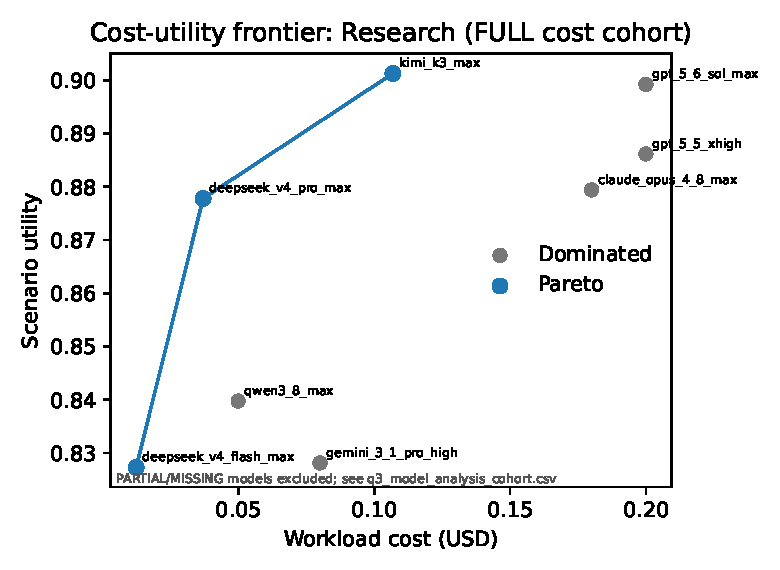
\includegraphics[width=\linewidth]{q3_cost_utility_Research.pdf}
\caption{Research}
\end{subfigure}
\begin{subfigure}{0.32\textwidth}
\centering
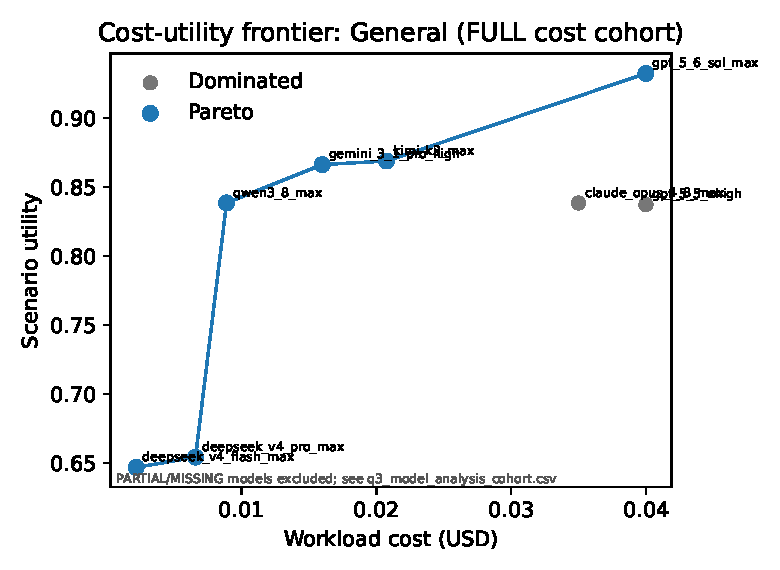
\includegraphics[width=\linewidth]{q3_cost_utility_General.pdf}
\caption{General}
\end{subfigure}
\begin{subfigure}{0.32\textwidth}
\centering
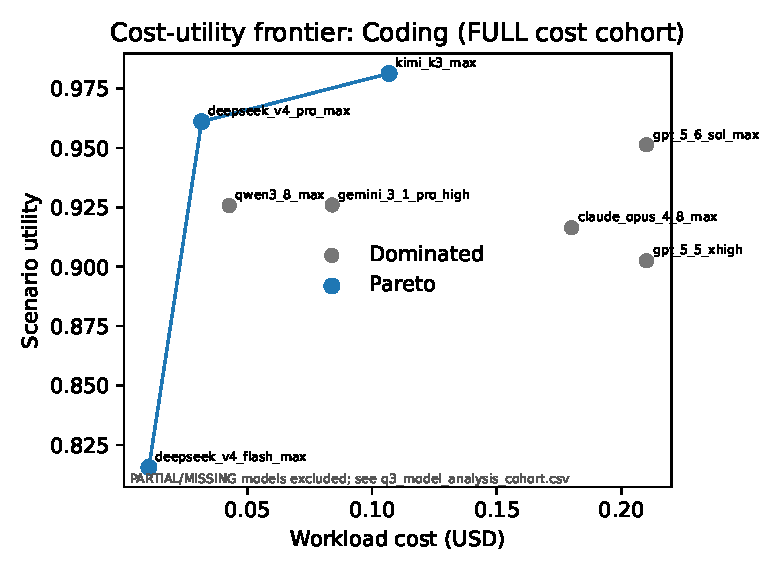
\includegraphics[width=\linewidth]{q3_cost_utility_Coding.pdf}
\caption{Coding}
\end{subfigure}
\caption{三类任务场景下模型效用--成本分布及 Pareto 有效前沿}
\label{fig:pareto}
\end{figure}

图 \ref{fig:pareto} 表明，最低成本模型在三个场景中均为
DeepSeek-V4-Flash Max，但前沿结构随场景效用变化而改变。Research 的
三个前沿点效用依次为 0.827289、0.877794 和 0.901293，对应成本为
0.012320、0.036960 和 0.106830 USD。Coding 的三个前沿点效用依次为
0.815577、0.961063 和 0.981302，对应成本为 0.010560、0.031680 和
0.106830 USD。

General 场景的前沿更长，依次包含 DeepSeek-V4-Flash Max、
DeepSeek-V4-Pro Max、Qwen3.8-Max、Gemini-3.1-Pro (High)、Kimi K3
和 GPT-5.6 Sol。其效用由 0.646876 提升至 0.932145，成本门槛由
0.002200 增至 0.040000 USD。相较之下，Research 和 Coding 中的部分
高价模型未带来足以抵消成本的效用优势，因而被 DeepSeek-V4-Pro Max 或
Kimi K3 支配。Fable 与 GLM 是进入严格比较前因成本不可观测而被排除，
不应表述为被 Pareto 支配。

\section{预算约束下的最优模型选择}

给定用户预算 $B$，定义场景 $s$ 下的最优可行模型为
\begin{equation}
i^*(B,s)=\arg\max_{i\in\mathcal M_{\mathrm{full}}}
U_i^{(s)}
\quad\text{s.t.}\quad C_i^{(s)}\le B.
\label{eq:budget}
\end{equation}
预算从低到高变化时，最优模型在 Pareto 模型的成本门槛处发生离散切换。
冻结结果如表 \ref{tab:budget} 所示。

\begin{table}[htbp]
\centering
\caption{三类场景预算约束下的最优模型切换}
\label{tab:budget}
\small
\begin{tabular}{llp{8.5cm}}
\toprule
场景 & 预算区间（USD） & 最优模型\\
\midrule
Research & $0.012320\le B<0.036960$ & DeepSeek-V4-Flash Max\\
Research & $0.036960\le B<0.106830$ & DeepSeek-V4-Pro Max\\
Research & $B\ge0.106830$ & Kimi K3\\
\midrule
General & $0.002200\le B<0.006600$ & DeepSeek-V4-Flash Max\\
General & $0.006600\le B<0.008903$ & DeepSeek-V4-Pro Max\\
General & $0.008903\le B<0.016000$ & Qwen3.8-Max\\
General & $0.016000\le B<0.020773$ & Gemini-3.1-Pro (High)\\
General & $0.020773\le B<0.040000$ & Kimi K3\\
General & $B\ge0.040000$ & GPT-5.6 Sol\\
\midrule
Coding & $0.010560\le B<0.031680$ & DeepSeek-V4-Flash Max\\
Coding & $0.031680\le B<0.106830$ & DeepSeek-V4-Pro Max\\
Coding & $B\ge0.106830$ & Kimi K3\\
\bottomrule
\end{tabular}
\end{table}

\begin{figure}[p]
\centering
\begin{subfigure}{0.32\textwidth}
\centering
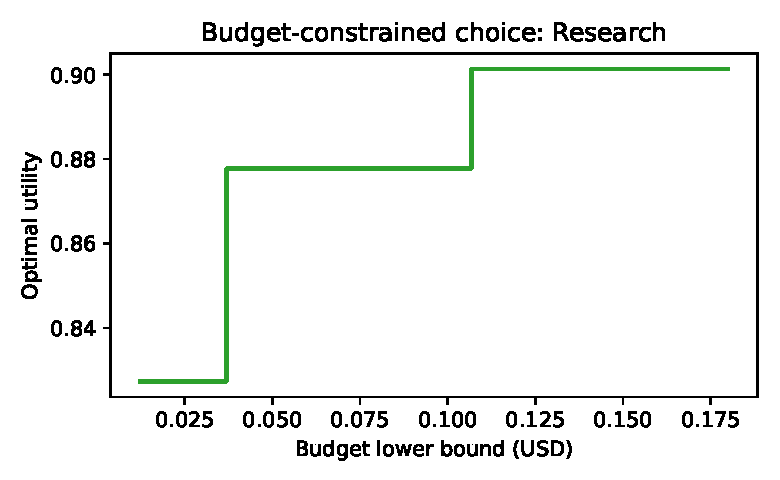
\includegraphics[width=\linewidth]{q3_budget_steps_Research.pdf}
\caption{Research}
\end{subfigure}
\begin{subfigure}{0.32\textwidth}
\centering
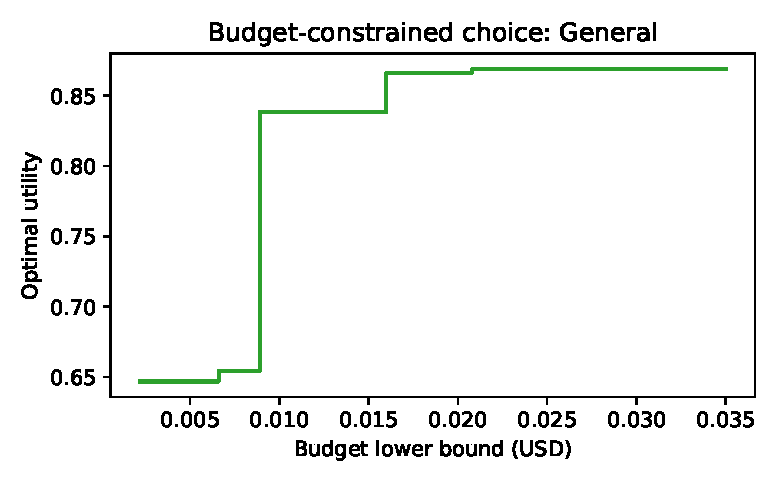
\includegraphics[width=\linewidth]{q3_budget_steps_General.pdf}
\caption{General}
\end{subfigure}
\begin{subfigure}{0.32\textwidth}
\centering
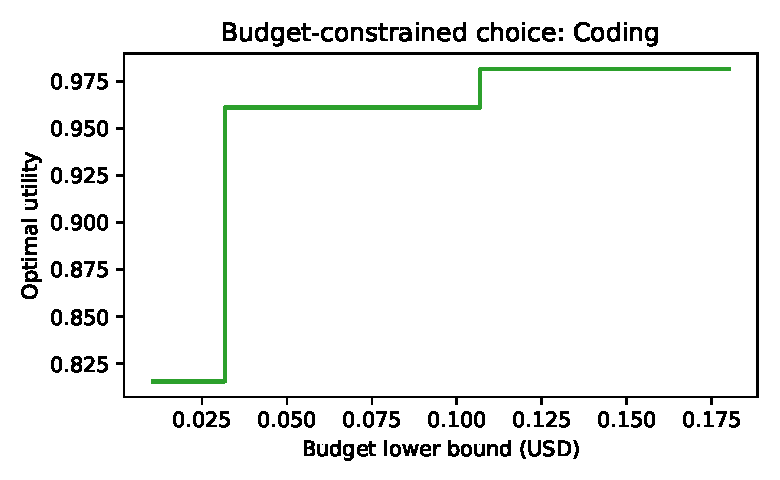
\includegraphics[width=\linewidth]{q3_budget_steps_Coding.pdf}
\caption{Coding}
\end{subfigure}
\caption{预算增加过程中的最优模型切换}
\label{fig:budget}
\end{figure}

\section{增量成本效益分析}

沿各场景 Pareto 前沿按成本升序排列，对相邻模型定义
\[
ICER_k=
\frac{C_{k+1}-C_k}{U_{k+1}-U_k}.
\]
该指标表示从当前有效模型升级到下一有效模型时，每增加一单位场景效用所
需承担的额外成本，并不等同于静态“性价比”。

\begin{table}[htbp]
\centering
\caption{Pareto 前沿相邻升级的增量成本效益}
\label{tab:icer}
\small
\begin{tabularx}{\textwidth}{lYYYYr}
\toprule
场景 & 当前模型 & 升级模型 & $\Delta C$ & $\Delta U$ & ICER\\
\midrule
Coding & DeepSeek Flash & DeepSeek Pro & 0.021120 & 0.145485 & 0.145169\\
Coding & DeepSeek Pro & Kimi K3 & 0.075150 & 0.020239 & 3.713059\\
General & DeepSeek Flash & DeepSeek Pro & 0.004400 & 0.007410 & 0.593761\\
General & DeepSeek Pro & Qwen3.8-Max & 0.002303 & 0.184094 & 0.012507\\
General & Qwen3.8-Max & Gemini Pro (High) & 0.007098 & 0.027779 & 0.255499\\
General & Gemini Pro (High) & Kimi K3 & 0.004772 & 0.002548 & 1.872844\\
General & Kimi K3 & GPT-5.6 Sol & 0.019228 & 0.063438 & 0.303089\\
Research & DeepSeek Flash & DeepSeek Pro & 0.024640 & 0.050504 & 0.487879\\
Research & DeepSeek Pro & Kimi K3 & 0.069870 & 0.023499 & 2.973325\\
\bottomrule
\end{tabularx}

\vspace{0.3em}
\footnotesize 注：成本单位为 USD，ICER 单位为 USD/utility。
\end{table}

Coding 和 Research 的末端升级分别需要 3.713059 和 2.973325 USD/utility，
显著高于前一段升级。这说明从 DeepSeek-V4-Pro Max 转向 Kimi K3 虽可继续
提高效用，但追加成本相对于效用增益较大。General 的前沿包含更多中间层级：
DeepSeek-V4-Pro Max 到 Qwen3.8-Max 的 ICER 仅为 0.012507，而
Gemini-3.1-Pro (High) 到 Kimi K3 的效用增量只有 0.002548，对应
1.872844 USD/utility，表现出明显不同的边际升级特征。

\section{成本--性能变化规律}

为避免仅依赖样本内拟合优度，分别对全体 FULL cohort 和 Pareto 子集比较
\[
U=a+bC,\qquad
U=a+b\ln(1+C),\qquad
U=a-be^{-kC}.
\]
评价指标包括 $R^2$、AIC、AICc、BIC 和留一交叉验证误差（LOOCV）。
全体 FULL cohort 的样本量为 $n=8$，因此 AICc 和 LOOCV 比单独使用
$R^2$ 更重要。

\begin{table}[htbp]
\centering
\caption{全体 FULL cohort 的成本--性能拟合摘要}
\label{tab:fit}
\small
\begin{tabular}{llrrrrr}
\toprule
场景 & 模型 & $R^2$ & AIC & AICc & BIC & LOOCV\\
\midrule
Research & Linear & 0.470986 & -57.794596 & -55.394596 & -57.635713 & 0.000682\\
Research & Log & 0.473763 & -57.836691 & -55.436691 & -57.677808 & 0.000678\\
Research & Saturation & 0.481753 & -55.959100 & -49.959100 & -55.720775 & 0.000870\\
General & Linear & 0.506858 & -39.042970 & -36.642970 & -38.884087 & 0.008176\\
General & Log & 0.509852 & -39.091699 & -36.691699 & -38.932816 & 0.008130\\
General & Saturation & 0.755203 & -42.645925 & -36.645925 & -42.407600 & 9.802600\\
Coding & Linear & 0.070341 & -45.508753 & -43.108753 & -45.349870 & 0.004055\\
Coding & Log & 0.077727 & -45.572561 & -43.172561 & -45.413677 & 0.004089\\
Coding & Saturation & 0.070329 & -43.508649 & -37.508649 & -43.270324 & 0.003159\\
\bottomrule
\end{tabular}
\end{table}

按 AICc，Research 和 Coding 的最优候选分别为 Log，General 的最优候选为
Saturation；按 LOOCV，Research 选择 Log，General 选择 Log，Coding 选择
Saturation。然而 General 的 Saturation LOOCV error 为 9.802600，远高于
Linear 和 Log，说明其样本内拟合优势并不具有稳定的外推表现。Research 和
Coding 的 Pareto 前沿只有 3 个点，前沿拟合因此标记为“前沿样本不足”。
综合样本规模、指标差异和前沿样本不足，当前数据没有提供跨场景统一的
成本边际收益递减规律证据。

\begin{figure}[p]
\centering
\begin{subfigure}{0.32\textwidth}
\centering
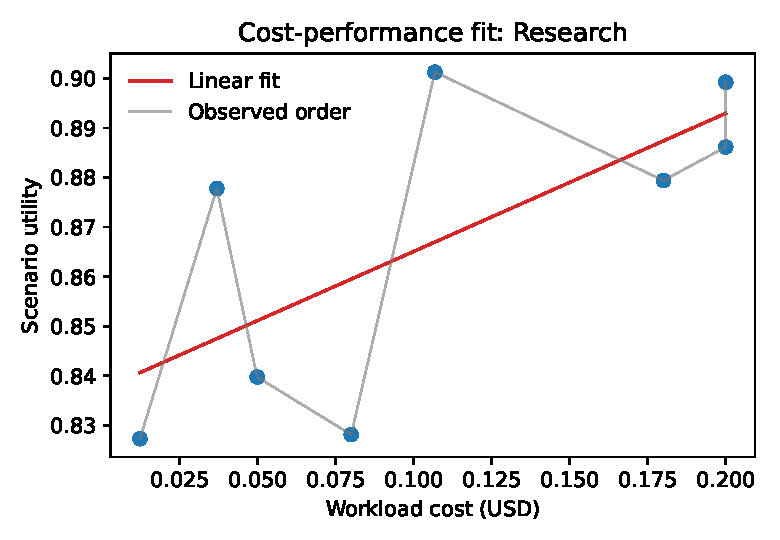
\includegraphics[width=\linewidth]{q3_cost_performance_fit_Research.pdf}
\caption{Research}
\end{subfigure}
\begin{subfigure}{0.32\textwidth}
\centering
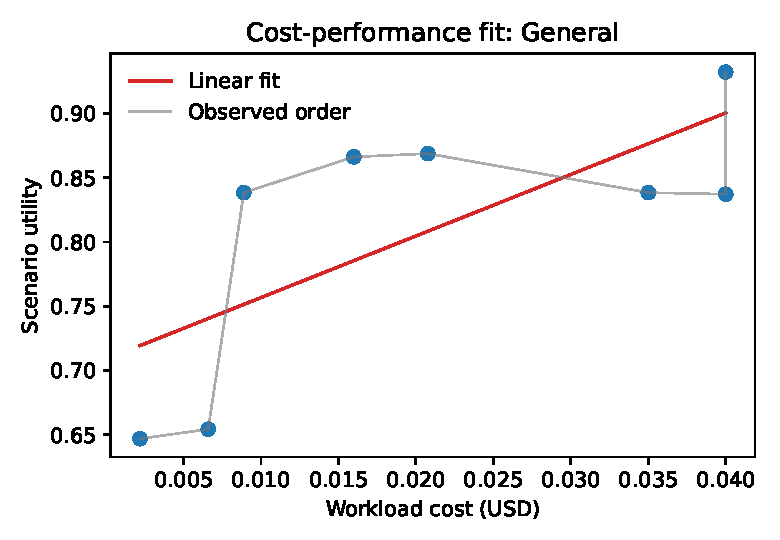
\includegraphics[width=\linewidth]{q3_cost_performance_fit_General.pdf}
\caption{General}
\end{subfigure}
\begin{subfigure}{0.32\textwidth}
\centering
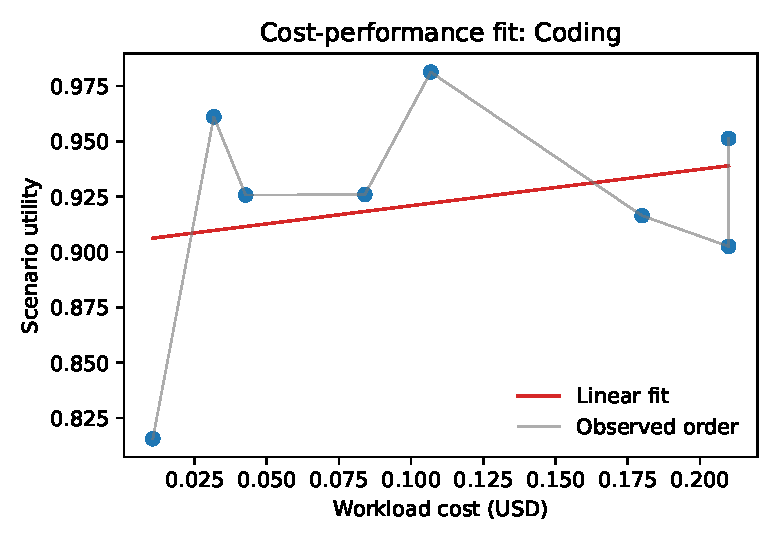
\includegraphics[width=\linewidth]{q3_cost_performance_fit_Coding.pdf}
\caption{Coding}
\end{subfigure}
\caption{全体 FULL cohort 的成本--性能拟合诊断}
\label{fig:fit}
\end{figure}

上述关系来自同一时间截面的模型性能与价格数据，只反映成本与场景效用
之间的统计关联，不构成成本导致性能提升的因果证据。

\section{敏感性与稳健性分析}

\subsection{工作负载与价格敏感性}

Q3 分别改变输入规模、输出/输入比例和价格，对成本排序、Pareto 成员及
预算切换进行检验。对三类场景的全部测试网格，nominal Pareto 成员保留率
和“全部 nominal 成员仍被保留”的比例均为 1.0000。输入规模测试点分别为
3 个，输出/输入比例测试点为 5 个，价格扰动测试点为 5 个；价格扰动采用
$-10\%,-5\%,0,+5\%,+10\%$。

当 $r=L_{\mathrm{out}}/L_{\mathrm{in}}$ 时，成本可写成
\[
C_i^{(s)}
=\frac{N_sL_{\mathrm{in}}^{(s)}}{10^6}
\left(p_{\mathrm{in},i}+r\,p_{\mathrm{out},i}\right).
\]
因此，任务由输入密集型转向输出密集型时，模型之间的成本差异会更多受到
输出单价影响。冻结敏感性结果显示，在本次标准化测试网格内，三类场景的
Pareto 结构均保持稳定；这一结论不延伸为对未观测生产负载或未来价格变化
的无条件保证。

\begin{figure}[p]
\centering
\begin{subfigure}{0.32\textwidth}
\centering
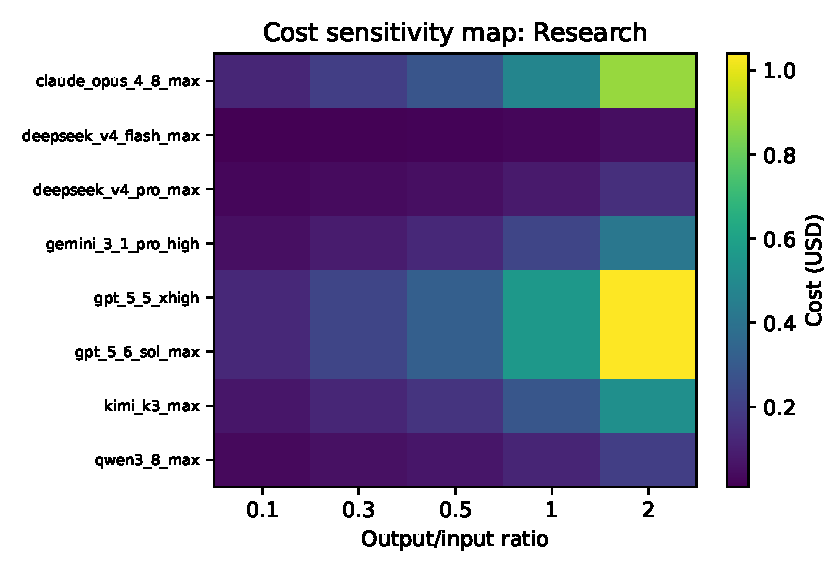
\includegraphics[width=\linewidth]{q3_ratio_sensitivity_Research.pdf}
\caption{Research}
\end{subfigure}
\begin{subfigure}{0.32\textwidth}
\centering
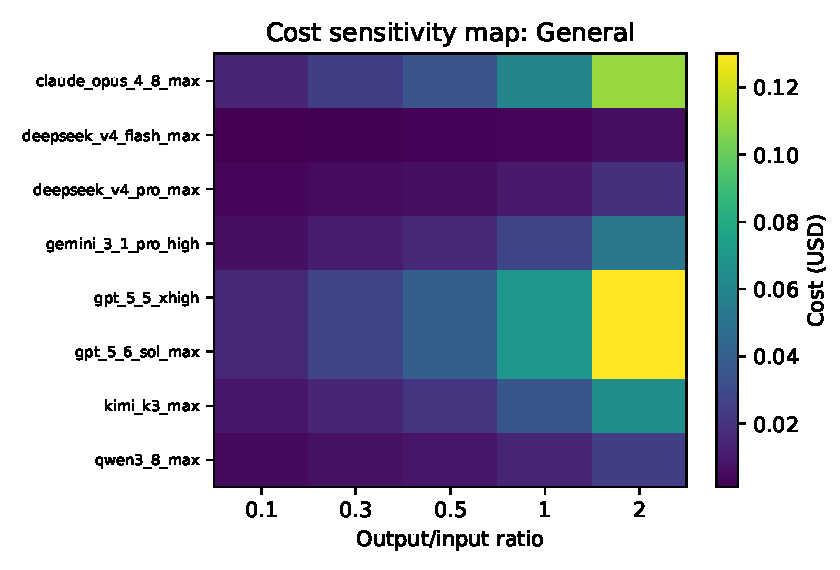
\includegraphics[width=\linewidth]{q3_ratio_sensitivity_General.pdf}
\caption{General}
\end{subfigure}
\begin{subfigure}{0.32\textwidth}
\centering
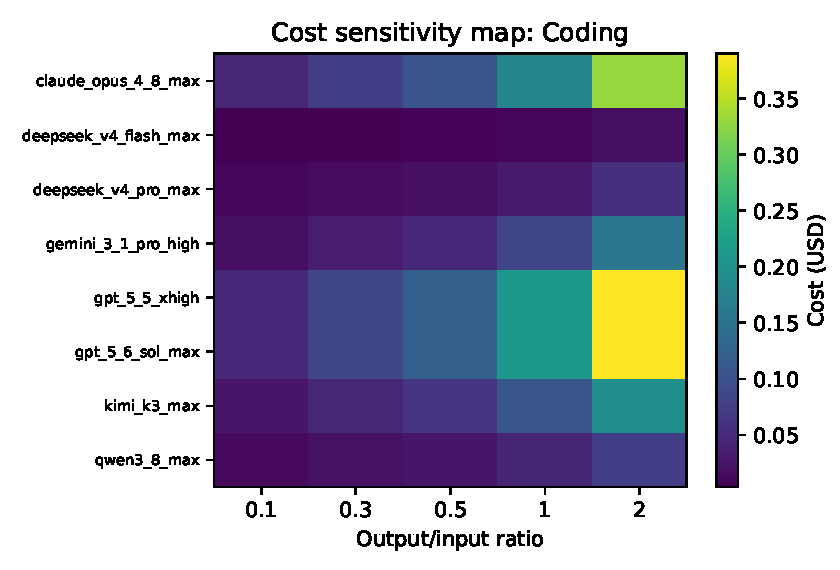
\includegraphics[width=\linewidth]{q3_ratio_sensitivity_Coding.pdf}
\caption{Coding}
\end{subfigure}
\caption{输入--输出比例变化下的 Pareto 结构}
\label{fig:ratio}
\end{figure}

\subsection{Bootstrap Pareto 稳定性}

Q2 已提供 2000 次 bootstrap 场景效用抽样。对每一次抽样 $b$，Q3 在固定
FULL cohort 成本下重新计算 Pareto 集合 $\mathcal P_s^{(b)}$，定义模型进入
前沿的概率为
\[
\pi_i^{(s)}
=\frac{1}{2000}\sum_{b=1}^{2000}
\mathbf 1\left(i\in\mathcal P_s^{(b)}\right).
\]
该概率刻画能力估计不确定性向 Q3 传播后，模型仍保持 Pareto 有效的频率。

\begin{table}[htbp]
\centering
\caption{Bootstrap Pareto 有效概率}
\label{tab:bootstrap}
\small
\begin{tabular}{lrrr}
\toprule
模型 & Research & General & Coding\\
\midrule
Claude Opus 4.8 & 0.0565 & 0.0400 & 0.0015\\
DeepSeek-V4-Flash Max & 1.0000 & 1.0000 & 1.0000\\
DeepSeek-V4-Pro Max & 0.8890 & 0.6745 & 0.9465\\
Gemini-3.1-Pro (High) & 0.1100 & 0.9050 & 0.1620\\
GPT-5.5 & 0.0335 & 0.0000 & 0.0000\\
GPT-5.6 Sol & 0.3405 & 0.9765 & 0.0600\\
Kimi K3 & 0.7355 & 0.5225 & 0.6150\\
Qwen3.8-Max & 0.1045 & 1.0000 & 0.2840\\
\bottomrule
\end{tabular}
\end{table}

Bootstrap 结果强化了若干 nominal 结论：DeepSeek-V4-Flash Max 在三个场景
中的 Pareto 概率均为 1.0000；DeepSeek-V4-Pro Max 在 Coding、General、
Research 中分别为 0.9465、0.6745、0.8890。General 场景的
Qwen3.8-Max 和 GPT-5.6 Sol 概率分别为 1.0000 和 0.9765，说明其在该
场景下的前沿地位较稳定。Kimi K3 在 Coding 中的概率为 0.6150，在
Research 和 General 中分别为 0.7355 和 0.5225，表现出更明显的边界
属性。Bootstrap 概率只传播 Q2 效用估计不确定性，没有覆盖价格更新、缓存、
峰谷时段、延迟、可用性或速率限制。

\begin{figure}[p]
\centering
\begin{subfigure}{0.32\textwidth}
\centering
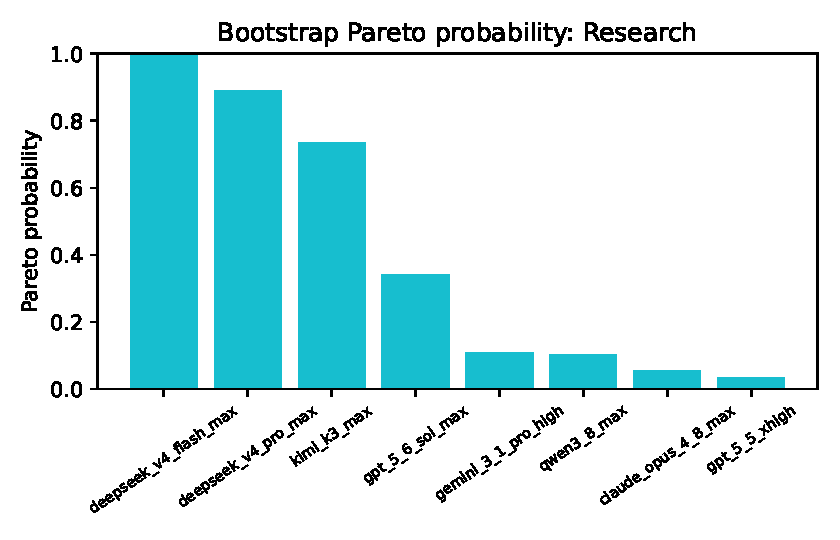
\includegraphics[width=\linewidth]{q3_pareto_probability_Research.pdf}
\caption{Research}
\end{subfigure}
\begin{subfigure}{0.32\textwidth}
\centering
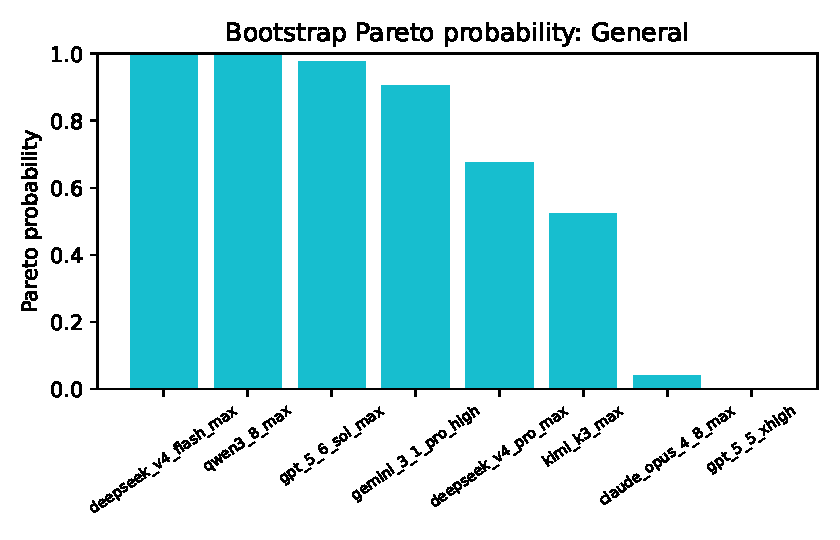
\includegraphics[width=\linewidth]{q3_pareto_probability_General.pdf}
\caption{General}
\end{subfigure}
\begin{subfigure}{0.32\textwidth}
\centering
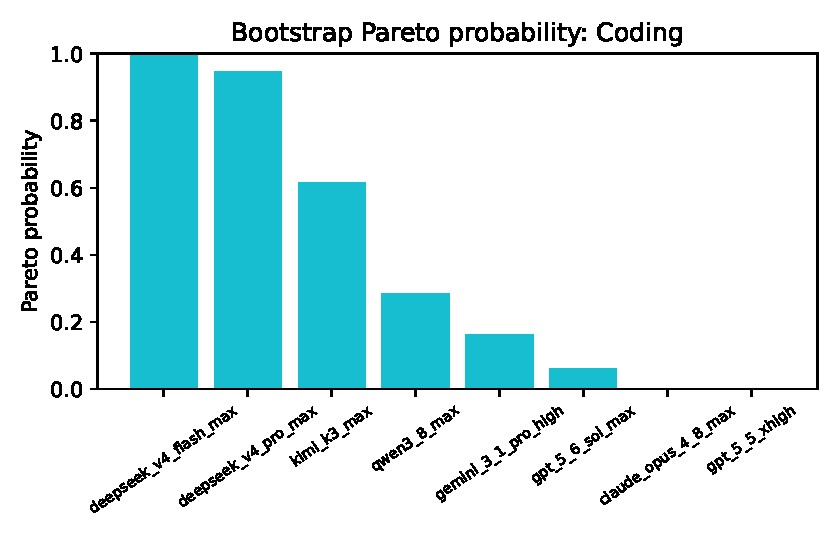
\includegraphics[width=\linewidth]{q3_pareto_probability_Coding.pdf}
\caption{Coding}
\end{subfigure}
\caption{Bootstrap 抽样下模型进入 Pareto 前沿的概率}
\label{fig:bootstrap}
\end{figure}

\section{问题三结果分析与小结}

本题的模型选型不能由一个脱离任务的“性能/价格”比值决定。场景工作负载
同时决定输入与输出 Token 的数量，Pareto 分析保留了成本和效用之间的
不可替代权衡，预算模型则将这种权衡转化为可以直接执行的切换规则。

综合冻结结果可得以下结论：
\begin{enumerate}[leftmargin=2.2em,itemsep=0.2em]
\item Research 和 Coding 的有效前沿均为 DeepSeek-V4-Flash Max、
DeepSeek-V4-Pro Max 和 Kimi K3；General 的前沿进一步包含 Qwen3.8-Max、
Gemini-3.1-Pro (High) 和 GPT-5.6 Sol。
\item DeepSeek-V4-Flash Max 在三个场景中都是最低成本的可行模型。随着
预算跨越表 \ref{tab:budget} 所列成本门槛，最优模型按 Pareto 前沿顺序
离散切换。
\item Coding 和 Research 从 DeepSeek-V4-Pro Max 升级至 Kimi K3 的 ICER
分别为 3.713059 和 2.973325 USD/utility，说明末端效用增益需要付出
较高追加成本；General 的中段升级则存在较低 ICER。
\item 全体 FULL cohort 的成本--性能拟合在不同场景间没有统一的稳定函数
形式。General 的饱和模型虽有较高 $R^2$，但 LOOCV error 为 9.802600，
不能据此断言普遍存在边际收益递减。
\item 在本次输入规模、输出/输入比例及价格扰动网格内，三类场景的 nominal
Pareto 成员均保持，说明冻结结论对已测试扰动具有稳健性。
\item Bootstrap 将 Q2 的 2000 次效用抽样传播至 Q3。Flash 在三个场景的
Pareto 概率均为 1.0000，General 中 Qwen3.8-Max 与 GPT-5.6 Sol 分别为
1.0000 和 0.9765；但该稳健性只针对效用估计不确定性。
\end{enumerate}

本研究的限制包括：API 价格具有时间变动性；标准化工作负载不覆盖所有真实
用户；Fable 的完整 fallback 成本和 GLM-5.2 的公开标准单价仍不可观测；
可比较模型数量有限；成本--性能拟合是横截面统计关联而非因果关系。因此，
本文结论应理解为在冻结价格、标准化工作负载和 FULL cohort 条件下的场景化
选型规则，而不是对所有生产环境的永久排名。

\section*{数据与价格来源说明}

本文使用问题二冻结的场景效用及其 bootstrap 接口，并使用 Q3 v1.0 冻结的
工作负载、价格核验和最终结果表。价格依据冻结审计中记录的官方模型与 API
文档，包括 OpenAI、Anthropic、Google、DeepSeek、Moonshot/Kimi、阿里云
百炼和智谱开放平台的官方资料；具体 SKU、配置、单价、日期和汇率信息以
冻结审计记录为准。Q3 冻结版本为 v1.0，Q2 接口采用正式冻结版本。

\end{document}
